
\documentclass[10pt,a4paper]{article}
\usepackage[T1]{fontenc}
\usepackage{tikz}
\usepackage[margin=1cm]{geometry}
\begin{document}

% Explanation about the algorithm
\section*{Binary Tree Search Algorithm}
In this document, we illustrate the process of searching for a value in a binary tree. The search algorithm is a depth-first search (DFS) using recursion, and it operates as follows:

\begin{enumerate}
    \item \textbf{Start at the Root:}
    Begin the search at the root of the binary tree.
    
    \item \textbf{Check Current Node:}
    Compare the value of the current node with the target value. If they match, the search is successful.

    \item \textbf{Recursive Search:}
    If the current node's value does not match the target, recursively search the left and right subtrees. This is done by calling the search function on the left child and then on the right child.

    \item \textbf{Highlighting Nodes:}
    During the search process, nodes being visited are highlighted to show their role in the search. If the target node is found, it is highlighted in purple.

    \item \textbf{End of Search:}
    The search concludes when the target value is found or all nodes have been visited. If the target is not found after traversing the entire tree, the search concludes with a failure.
\end{enumerate}

% Detailed Steps
\section*{Detailed Steps}
The following figures illustrate the binary tree at various stages of the search process. Each figure shows the state of the tree at different points during the search operation.


\begin{figure}[h!]
\centering

\begin{minipage}{0.8\textwidth}
    \centering
    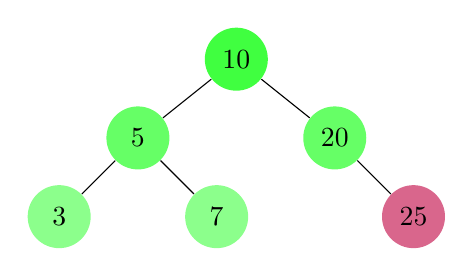
\begin{tikzpicture}[level distance=10mm]
        \tikzstyle{every node}=[fill=green!75,circle,inner sep=1pt, minimum size=8mm]
        \tikzstyle{level 1}=[sibling distance=25mm, set style={{every node}+=[fill=green!60]}]
        \tikzstyle{level 2}=[sibling distance=20mm, set style={{every node}+=[fill=green!45]}]
        \tikzstyle{level 3}=[sibling distance=15mm, set style={{every node}+=[fill=green!30]}]
        \tikzstyle{level 4}=[sibling distance=10mm, set style={{every node}+=[fill=green!15]}]
        \node {10} child {node {5} child {node {3} } child {node {7} }} child {node {20} child[fill=none] {edge from parent[draw=none]} child {node[fill=purple!60] {25} }};
    \end{tikzpicture}
    \caption{Step 1}
\end{minipage}
\vspace{1cm}

\begin{minipage}{0.8\textwidth}
    \centering
    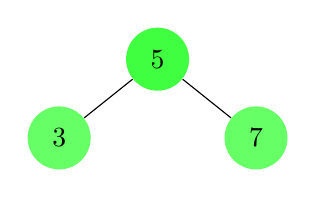
\begin{tikzpicture}[level distance=10mm]
        \tikzstyle{every node}=[fill=green!75,circle,inner sep=1pt, minimum size=8mm]
        \tikzstyle{level 1}=[sibling distance=25mm, set style={{every node}+=[fill=green!60]}]
        \tikzstyle{level 2}=[sibling distance=20mm, set style={{every node}+=[fill=green!45]}]
        \tikzstyle{level 3}=[sibling distance=15mm, set style={{every node}+=[fill=green!30]}]
        \tikzstyle{level 4}=[sibling distance=10mm, set style={{every node}+=[fill=green!15]}]
        \node {5} child {node {3} } child {node {7} };
    \end{tikzpicture}
    \caption{Step 2}
\end{minipage}
\vspace{1cm}

\begin{minipage}{0.8\textwidth}
    \centering
    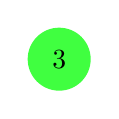
\begin{tikzpicture}[level distance=10mm]
        \tikzstyle{every node}=[fill=green!75,circle,inner sep=1pt, minimum size=8mm]
        \tikzstyle{level 1}=[sibling distance=25mm, set style={{every node}+=[fill=green!60]}]
        \tikzstyle{level 2}=[sibling distance=20mm, set style={{every node}+=[fill=green!45]}]
        \tikzstyle{level 3}=[sibling distance=15mm, set style={{every node}+=[fill=green!30]}]
        \tikzstyle{level 4}=[sibling distance=10mm, set style={{every node}+=[fill=green!15]}]
        \node {3} ;
    \end{tikzpicture}
    \caption{Step 3}
\end{minipage}
\vspace{1cm}

\begin{minipage}{0.8\textwidth}
    \centering
    
\begin{tikzpicture}[level distance=10mm]
        \tikzstyle{every node}=[fill=green!75,circle,inner sep=1pt, minimum size=8mm]
        \tikzstyle{level 1}=[sibling distance=25mm, set style={{every node}+=[fill=green!60]}]
        \tikzstyle{level 2}=[sibling distance=20mm, set style={{every node}+=[fill=green!45]}]
        \tikzstyle{level 3}=[sibling distance=15mm, set style={{every node}+=[fill=green!30]}]
        \tikzstyle{level 4}=[sibling distance=10mm, set style={{every node}+=[fill=green!15]}]
        \node {7} ;
    \end{tikzpicture}
    \caption{Step 4}
\end{minipage}
\vspace{1cm}

\begin{minipage}{0.8\textwidth}
    \centering
    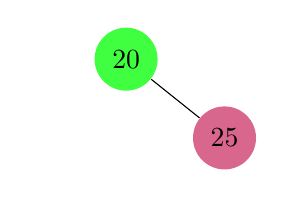
\begin{tikzpicture}[level distance=10mm]
        \tikzstyle{every node}=[fill=green!75,circle,inner sep=1pt, minimum size=8mm]
        \tikzstyle{level 1}=[sibling distance=25mm, set style={{every node}+=[fill=green!60]}]
        \tikzstyle{level 2}=[sibling distance=20mm, set style={{every node}+=[fill=green!45]}]
        \tikzstyle{level 3}=[sibling distance=15mm, set style={{every node}+=[fill=green!30]}]
        \tikzstyle{level 4}=[sibling distance=10mm, set style={{every node}+=[fill=green!15]}]
        \node {20} child[fill=none] {edge from parent[draw=none]} child {node[fill=purple!60] {25} };
    \end{tikzpicture}
    \caption{Step 5}
\end{minipage}
\vspace{1cm}

\begin{minipage}{0.8\textwidth}
    \centering
    
\begin{tikzpicture}[level distance=10mm]
        \tikzstyle{every node}=[fill=green!75,circle,inner sep=1pt, minimum size=8mm]
        \tikzstyle{level 1}=[sibling distance=25mm, set style={{every node}+=[fill=green!60]}]
        \tikzstyle{level 2}=[sibling distance=20mm, set style={{every node}+=[fill=green!45]}]
        \tikzstyle{level 3}=[sibling distance=15mm, set style={{every node}+=[fill=green!30]}]
        \tikzstyle{level 4}=[sibling distance=10mm, set style={{every node}+=[fill=green!15]}]
        \node[fill=purple!60] {25} ;
    \end{tikzpicture}
    \caption{Step 6}
\end{minipage}
\vspace{1cm}

\end{figure}
\newpage

\end{document}
